\documentclass{standalone}
\usepackage{tikz}
\usetikzlibrary{patterns, positioning}
\usetikzlibrary{shapes.misc}
\usepackage[outline]{contour}
\contourlength{1.5pt} 


\begin{document}
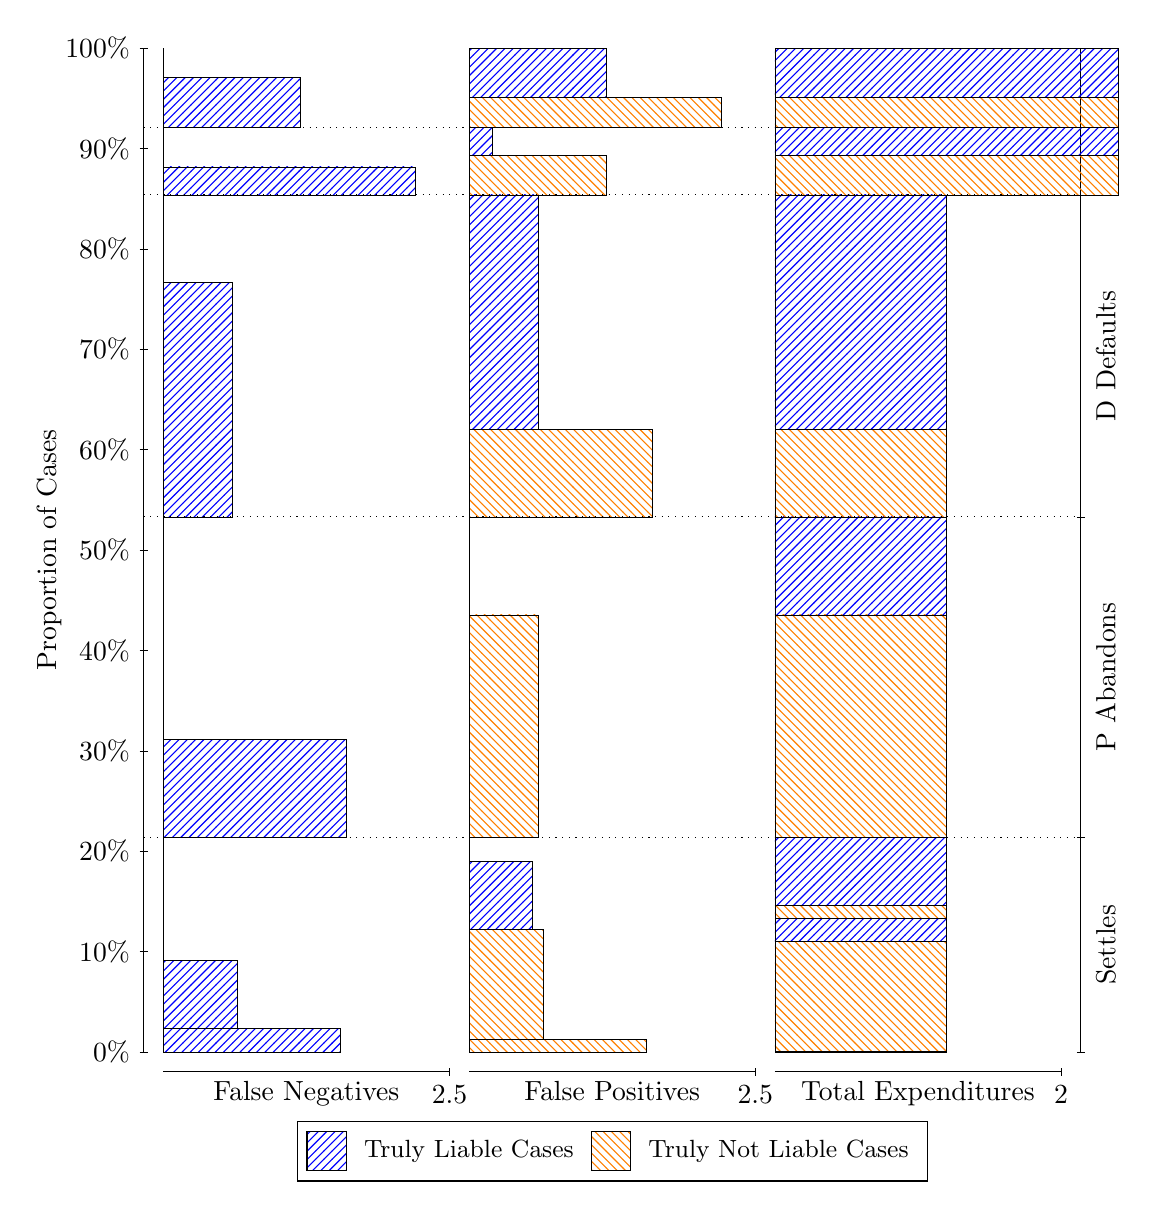
\begin{tikzpicture}
\draw[black, very thin] (1.5,1.75) -- (1.5,14.5);
\node[rotate=90, text=black, anchor=center] at (0.3, 8.125) {Proportion of Cases};
\draw[black, very thin] (1.45,1.75) -- (1.55,1.75);
\node[text=black, anchor=east] at (1.45, 1.75) {0\%};
\draw[black, very thin] (1.45,3.025) -- (1.55,3.025);
\node[text=black, anchor=east] at (1.45, 3.025) {10\%};
\draw[black, very thin] (1.45,4.3) -- (1.55,4.3);
\node[text=black, anchor=east] at (1.45, 4.3) {20\%};
\draw[black, very thin] (1.45,5.575) -- (1.55,5.575);
\node[text=black, anchor=east] at (1.45, 5.575) {30\%};
\draw[black, very thin] (1.45,6.85) -- (1.55,6.85);
\node[text=black, anchor=east] at (1.45, 6.85) {40\%};
\draw[black, very thin] (1.45,8.125) -- (1.55,8.125);
\node[text=black, anchor=east] at (1.45, 8.125) {50\%};
\draw[black, very thin] (1.45,9.4) -- (1.55,9.4);
\node[text=black, anchor=east] at (1.45, 9.4) {60\%};
\draw[black, very thin] (1.45,10.675) -- (1.55,10.675);
\node[text=black, anchor=east] at (1.45, 10.675) {70\%};
\draw[black, very thin] (1.45,11.95) -- (1.55,11.95);
\node[text=black, anchor=east] at (1.45, 11.95) {80\%};
\draw[black, very thin] (1.45,13.225) -- (1.55,13.225);
\node[text=black, anchor=east] at (1.45, 13.225) {90\%};
\draw[black, very thin] (1.45,14.5) -- (1.55,14.5);
\node[text=black, anchor=east] at (1.45, 14.5) {100\%};

\draw[black, very thin] (13.4,1.75) -- (13.4,14.5);
\draw[black, very thin] (13.35,1.75) -- (13.45,1.75);
\node[anchor=west] at (13.35, 1.75) {};
\draw[black, very thin] (13.35,4.4715) -- (13.45,4.4715);
\node[anchor=west] at (13.35, 4.4715) {};
\draw[black, very thin] (13.35,8.5458) -- (13.45,8.5458);
\node[anchor=west] at (13.35, 8.5458) {};
\draw[black, very thin] (13.35,12.636) -- (13.45,12.636);
\node[anchor=west] at (13.35, 12.636) {};
\draw[black, very thin] (13.35,13.493) -- (13.45,13.493);
\node[anchor=west] at (13.35, 13.493) {};
\draw[black, very thin] (13.35,14.5) -- (13.45,14.5);
\node[anchor=west] at (13.35, 14.5) {};

\draw[black, very thin, pattern color=blue, pattern=north east lines] (1.75,1.75) rectangle (4.0027,2.0467);
\draw[black, very thin, pattern color=blue, pattern=north east lines] (1.75,2.0467) rectangle (3.3487,2.0486);
\draw[black, very thin, pattern color=blue, pattern=north east lines] (1.75,2.0486) rectangle (2.6947,2.9111);
\draw[black, very thin, pattern color=orange, pattern=north west lines] (1.75,2.9111) rectangle (1.75,4.4715);
\draw[black, very thin, pattern color=blue, pattern=north east lines] (1.75,4.4715) rectangle (4.0753,5.7176);
\draw[black, very thin, pattern color=orange, pattern=north west lines] (1.75,5.7176) rectangle (1.75,8.5458);
\draw[black, very thin, pattern color=blue, pattern=north east lines] (1.75,8.5458) rectangle (2.622,11.528);
\draw[black, very thin, pattern color=orange, pattern=north west lines] (1.75,11.528) rectangle (1.75,12.636);
\draw[black, very thin, pattern color=blue, pattern=north east lines] (1.75,12.636) rectangle (4.9473,12.99);
\draw[black, very thin, pattern color=orange, pattern=north west lines] (1.75,12.99) rectangle (1.75,13.493);
\draw[black, very thin, pattern color=blue, pattern=north east lines] (1.75,13.493) rectangle (3.494,14.124);
\draw[black, very thin, pattern color=orange, pattern=north west lines] (1.75,14.124) rectangle (1.75,14.5);
\draw[black, very thin, pattern color=orange, pattern=north west lines] (5.6333,1.75) rectangle (7.886,1.9097);
\draw[black, very thin, pattern color=orange, pattern=north west lines] (5.6333,1.9097) rectangle (7.232,1.9113);
\draw[black, very thin, pattern color=orange, pattern=north west lines] (5.6333,1.9113) rectangle (6.578,3.3104);
\draw[black, very thin, pattern color=blue, pattern=north east lines] (5.6333,3.3104) rectangle (6.4327,4.1729);
\draw[black, very thin, pattern color=blue, pattern=north east lines] (5.6333,4.1729) rectangle (5.7787,4.1748);
\draw[black, very thin, pattern color=blue, pattern=north east lines] (5.6333,4.1748) rectangle (5.6333,4.4715);
\draw[black, very thin, pattern color=orange, pattern=north west lines] (5.6333,4.4715) rectangle (6.5053,7.2996);
\draw[black, very thin, pattern color=blue, pattern=north east lines] (5.6333,7.2996) rectangle (5.6333,8.5458);
\draw[black, very thin, pattern color=orange, pattern=north west lines] (5.6333,8.5458) rectangle (7.9587,9.6538);
\draw[black, very thin, pattern color=blue, pattern=north east lines] (5.6333,9.6538) rectangle (6.5053,12.636);
\draw[black, very thin, pattern color=orange, pattern=north west lines] (5.6333,12.636) rectangle (7.3773,13.139);
\draw[black, very thin, pattern color=blue, pattern=north east lines] (5.6333,13.139) rectangle (5.924,13.493);
\draw[black, very thin, pattern color=orange, pattern=north west lines] (5.6333,13.493) rectangle (8.8307,13.869);
\draw[black, very thin, pattern color=blue, pattern=north east lines] (5.6333,13.869) rectangle (7.3773,14.5);
\draw[black, very thin, pattern color=orange, pattern=north west lines] (9.5167,1.75) rectangle (11.697,1.7516);
\draw[black, very thin, pattern color=blue, pattern=north east lines] (9.5167,1.7516) rectangle (11.697,1.7535);
\draw[black, very thin, pattern color=orange, pattern=north west lines] (9.5167,1.7535) rectangle (11.697,3.1526);
\draw[black, very thin, pattern color=blue, pattern=north east lines] (9.5167,3.1526) rectangle (11.697,3.4493);
\draw[black, very thin, pattern color=orange, pattern=north west lines] (9.5167,3.4493) rectangle (11.697,3.609);
\draw[black, very thin, pattern color=blue, pattern=north east lines] (9.5167,3.609) rectangle (11.697,4.4715);
\draw[black, very thin, pattern color=orange, pattern=north west lines] (9.5167,4.4715) rectangle (11.697,7.2996);
\draw[black, very thin, pattern color=blue, pattern=north east lines] (9.5167,7.2996) rectangle (11.697,8.5458);
\draw[black, very thin, pattern color=orange, pattern=north west lines] (9.5167,8.5458) rectangle (11.697,9.6538);
\draw[black, very thin, pattern color=blue, pattern=north east lines] (9.5167,9.6538) rectangle (11.697,12.636);
\draw[black, very thin, pattern color=orange, pattern=north west lines] (9.5167,12.636) rectangle (13.877,13.139);
\draw[black, very thin, pattern color=blue, pattern=north east lines] (9.5167,13.139) rectangle (13.877,13.493);
\draw[black, very thin, pattern color=orange, pattern=north west lines] (9.5167,13.493) rectangle (13.877,13.869);
\draw[black, very thin, pattern color=blue, pattern=north east lines] (9.5167,13.869) rectangle (13.877,14.5);
\draw[black, dotted] (1.5,4.4715) -- (13.4,4.4715);
\draw[black, dotted] (1.5,8.5458) -- (13.4,8.5458);
\draw[black, dotted] (1.5,12.636) -- (13.4,12.636);
\draw[black, dotted] (1.5,13.493) -- (13.4,13.493);
\draw[black, very thin] (1.75,1.5) -- (5.3833,1.5);
\node[text=black, anchor=north] at (3.5667, 1.5) {False Negatives};
\draw[black, very thin] (5.3833,1.45) -- (5.3833,1.55);
\node[text=black, anchor=north] at (5.3833, 1.45) {2.5};

\draw[black, very thin] (5.6333,1.5) -- (9.2667,1.5);
\node[text=black, anchor=north] at (7.45, 1.5) {False Positives};
\draw[black, very thin] (9.2667,1.45) -- (9.2667,1.55);
\node[text=black, anchor=north] at (9.2667, 1.45) {2.5};

\draw[black, very thin] (9.5167,1.5) -- (13.15,1.5);
\node[text=black, anchor=north] at (11.333, 1.5) {Total Expenditures};
\draw[black, very thin] (13.15,1.45) -- (13.15,1.55);
\node[text=black, anchor=north] at (13.15, 1.45) {2};

\node[text=black, centered, rotate=90] at (13.72, 3.1107) {\contour{white}{Settles}};
\node[text=black, centered, rotate=90] at (13.72, 6.5086) {\contour{white}{P Abandons}};
\node[text=black, centered, rotate=90] at (13.72, 10.591) {\contour{white}{D Defaults}};



\draw (7.449999999999999,1.5) node[draw=none] (baseCoordinate) {};
\begin{scope}[align=center]
        \matrix[scale=0.5, draw=black, below=0.5cm of baseCoordinate, nodes={draw}, column sep=0.1cm]{
            \node[rectangle, draw, minimum width=0.5cm, minimum height=0.5cm, pattern color=blue, pattern=north east lines] {}; &
            \node[draw=none, font=\small, text=black] (B) {Truly Liable Cases}; &
            \node[rectangle, draw, minimum width=0.5cm, minimum height=0.5cm, pattern color=orange, pattern=north west lines] {}; &
            \node[draw=none, font=\small, text=black] (B) {Truly Not Liable Cases}; \\
            };
\end{scope}

\end{tikzpicture}
\end{document}